% !TeX root = ../main.tex

\section{Error Analysis and Discussion}


\begin{figure*}[!t]
\centering
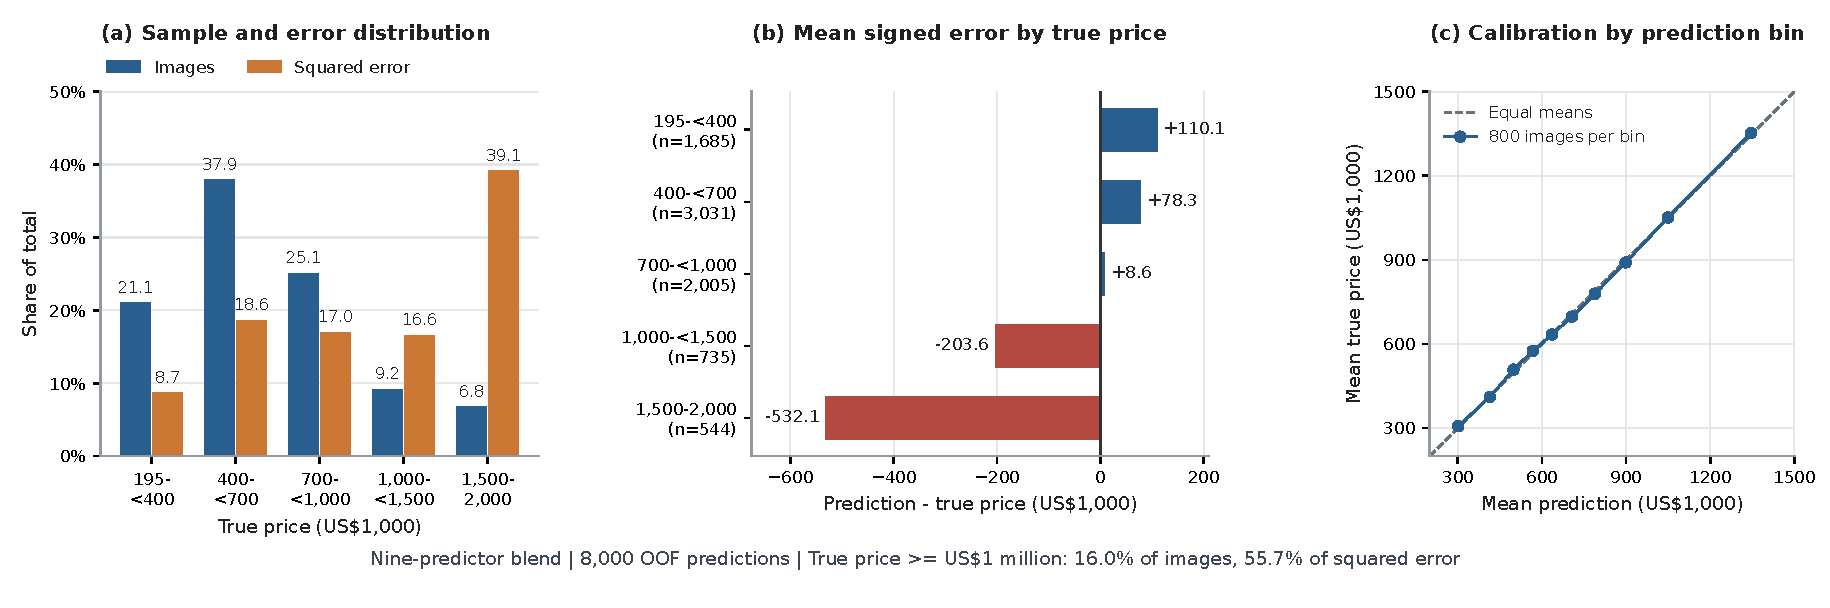
\includegraphics[width=\textwidth]{figure1_ensemble_error_analysis.pdf}
\caption{Error and calibration diagnostics for the final ensemble: (a) sample and squared-error shares by price band; (b) mean prediction bias; and (c) calibration across prediction bins, each holding 800 images. Bin means near the diagonal do not imply accurate estimates for individual images.}
\label{fig:diagnostics}
\end{figure*}

\begin{figure*}[!t]
\centering
\begin{minipage}[t]{0.24\textwidth}
\centering\footnotesize
\textbf{(a) 4244.jpg}\\
\parbox[c][2.1\baselineskip][c]{\linewidth}{\centering\textbf{Near-accurate}}
\par\smallskip
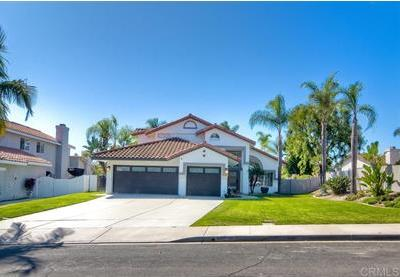
\includegraphics[width=\linewidth,height=32mm,keepaspectratio]{cases/4244.jpg}
\par\smallskip
True: 769.00\\
Predicted: 768.98\\
Error: \ensuremath{-}0.02
\end{minipage}
\hfill
\begin{minipage}[t]{0.24\textwidth}
\centering\footnotesize
\textbf{(b) 2138.jpg}\\
\parbox[c][2.1\baselineskip][c]{\linewidth}{\centering\textbf{Severe underestimate}}
\par\smallskip
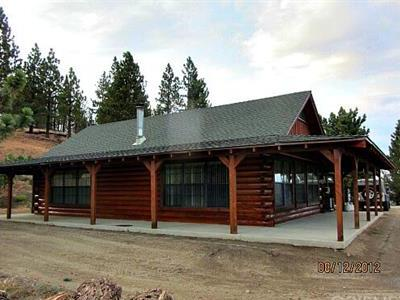
\includegraphics[width=\linewidth,height=32mm,keepaspectratio]{cases/2138.jpg}
\par\smallskip
True: 1,995.00\\
Predicted: 526.61\\
Error: \ensuremath{-}1,468.39
\end{minipage}
\hfill
\begin{minipage}[t]{0.24\textwidth}
\centering\footnotesize
\textbf{(c) 5350.jpg}\\
\parbox[c][2.1\baselineskip][c]{\linewidth}{\centering\textbf{Overestimate}}
\par\smallskip
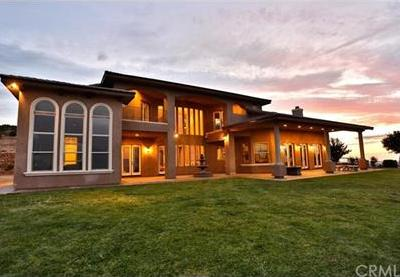
\includegraphics[width=\linewidth,height=32mm,keepaspectratio]{cases/5350.jpg}
\par\smallskip
True: 635.00\\
Predicted: 1,485.39\\
Error: +850.39
\end{minipage}
\hfill
\begin{minipage}[t]{0.24\textwidth}
\centering\footnotesize
\textbf{(d) 2409.jpg}\\
\parbox[c][2.1\baselineskip][c]{\linewidth}{\centering\textbf{Partial tree occlusion}}
\par\smallskip
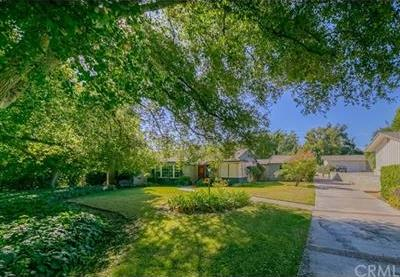
\includegraphics[width=\linewidth,height=32mm,keepaspectratio]{cases/2409.jpg}
\par\smallskip
True: 1,980.00\\
Predicted: 1,176.47\\
Error: \ensuremath{-}803.53
\end{minipage}
\par\medskip{\footnotesize Nine-predictor NNLS blend; OOF predictions; all values in US\$1,000.}
\caption{Four illustrative predictions from the final ensemble, showing a near-accurate estimate, a severe underestimate, an overestimate, and a case with foreground tree occlusion. These are individual examples rather than the overall distribution, and visible image characteristics cannot establish the causes of errors.}
\label{fig:cases}
\end{figure*}

% Typeset from reportdraft.en.md; edit this TeX file for subsequent revisions.

A lower overall error does not mean uniform improvement across price bands. Expensive houses dominate the MSE: the 1,279 images with true prices of at least 1,000 thousand dollars account for 16.0\% of the samples but contribute 55.7\% of the total squared error; there is also a clear direction of bias: the mean ``prediction minus true price'' bias in the 1,500--2,000 thousand dollar band is \ensuremath{-}532.1 thousand dollars, compared with +8.6 thousand dollars in the 700--1,000 band (Fig.~\ref{fig:diagnostics}).


Panels (b) and (c) of Fig.~\ref{fig:diagnostics} group the same predictions in two different ways and should not be read as one statement. Conditioning on the true price, as in (b), makes a predictor with limited information appear biased even when nothing is wrong with it: among houses that happen to be expensive, those the model cannot identify pull the group average down. Panel (c) conditions on the prediction instead, and all ten bins lie close to the diagonal, so the shrinkage in (b) appears calibrated rather than correctable: scaling the high end upwards would move predictions away from the conditional mean that squared error rewards, and the remaining tail error points to how little a photograph reveals about price band.


To further illustrate these MSEs, we show four specific cases from the final model (Fig.~\ref{fig:cases}). The facade in 4244.jpg is clear and its prediction of 768.98 is close to the true 769, which serves as an accurate reference. 2138.jpg is underestimated by 1468, possibly because its wooden exterior walls and sparse surrounding greenery do not reflect its higher true price. 5350.jpg is overestimated by 850, possibly because its tall arched windows, warm lighting and lawn are associated with higher-value houses. In 2409.jpg, there is considerable occlusion from trees in the foreground, which affected the model's judgement of the building's price.


In addition, this study was limited by available compute and runtime, which is also why we mainly used frozen visual features. Fine-tuning the visual encoder, to test whether an adapted representation separates price bands better than a general-purpose one, is therefore the main avenue we were unable to explore.
